
%% bare_jrnl_transmag.tex
%% V1.4a
%% 2014/09/17
%% by Michael Shell
%% see http://www.michaelshell.org/
%% for current contact information.
%%
%% This is a skeleton file demonstrating the use of IEEEtran.cls
%% (requires IEEEtran.cls version 1.8a or later) with an IEEE 
%% Transactions on Magnetics journal paper.
%%
%% Support sites:
%% http://www.michaelshell.org/tex/ieeetran/
%% http://www.ctan.org/tex-archive/macros/latex/contrib/IEEEtran/
%% and
%% http://www.ieee.org/

%%*************************************************************************
%% Legal Notice:
%% This code is offered as-is without any warranty either expressed or
%% implied; without even the implied warranty of MERCHANTABILITY or
%% FITNESS FOR A PARTICULAR PURPOSE! 
%% User assumes all risk.
%% In no event shall IEEE or any contributor to this code be liable for
%% any damages or losses, including, but not limited to, incidental,
%% consequential, or any other damages, resulting from the use or misuse
%% of any information contained here.
%%
%% All comments are the opinions of their respective authors and are not
%% necessarily endorsed by the IEEE.
%%
%% This work is distributed under the LaTeX Project Public License (LPPL)
%% ( http://www.latex-project.org/ ) version 1.3, and may be freely used,
%% distributed and modified. A copy of the LPPL, version 1.3, is included
%% in the base LaTeX documentation of all distributions of LaTeX released
%% 2003/12/01 or later.
%% Retain all contribution notices and credits.
%% ** Modified files should be clearly indicated as such, including  **
%% ** renaming them and changing author support contact information. **
%%
%% File list of work: IEEEtran.cls, IEEEtran_HOWTO.pdf, bare_adv.tex,
%%                    bare_conf.tex, bare_jrnl.tex, bare_conf_compsoc.tex,
%%                    bare_jrnl_compsoc.tex, bare_jrnl_transmag.tex
%%*************************************************************************


% *** Authors should verify (and, if needed, correct) their LaTeX system  ***
% *** with the testflow diagnostic prior to trusting their LaTeX platform ***
% *** with production work. IEEE's font choices and paper sizes can       ***
% *** trigger bugs that do not appear when using other class files.       ***                          ***
% The testflow support page is at:
% http://www.michaelshell.org/tex/testflow/



\documentclass[journal,transmag,twoside]{IEEEtran}
%
% If IEEEtran.cls has not been installed into the LaTeX system files,
% manually specify the path to it like:
% \documentclass[journal]{../sty/IEEEtran}





% Some very useful LaTeX packages include:
% (uncomment the ones you want to load)


% *** MISC UTILITY PACKAGES ***
%
%\usepackage{ifpdf}
% Heiko Oberdiek's ifpdf.sty is very useful if you need conditional
% compilation based on whether the output is pdf or dvi.
% usage:
% \ifpdf
%   % pdf code
% \else
%   % dvi code
% \fi
% The latest version of ifpdf.sty can be obtained from:
% http://www.ctan.org/tex-archive/macros/latex/contrib/oberdiek/
% Also, note that IEEEtran.cls V1.7 and later provides a builtin
% \ifCLASSINFOpdf conditional that works the same way.
% When switching from latex to pdflatex and vice-versa, the compiler may
% have to be run twice to clear warning/error messages.






% *** CITATION PACKAGES ***
%
%\usepackage{cite}
% cite.sty was written by Donald Arseneau
% V1.6 and later of IEEEtran pre-defines the format of the cite.sty package
% \cite{} output to follow that of IEEE. Loading the cite package will
% result in citation numbers being automatically sorted and properly
% "compressed/ranged". e.g., [1], [9], [2], [7], [5], [6] without using
% cite.sty will become [1], [2], [5]--[7], [9] using cite.sty. cite.sty's
% \cite will automatically add leading space, if needed. Use cite.sty's
% noadjust option (cite.sty V3.8 and later) if you want to turn this off
% such as if a citation ever needs to be enclosed in parenthesis.
% cite.sty is already installed on most LaTeX systems. Be sure and use
% version 5.0 (2009-03-20) and later if using hyperref.sty.
% The latest version can be obtained at:
% http://www.ctan.org/tex-archive/macros/latex/contrib/cite/
% The documentation is contained in the cite.sty file itself.






% *** GRAPHICS RELATED PACKAGES ***
%
\ifCLASSINFOpdf
  \usepackage[pdftex]{graphicx}
  % declare the path(s) where your graphic files are
  % \graphicspath{{../pdf/}{../jpeg/}}
  % and their extensions so you won't have to specify these with
  % every instance of \includegraphics
  % \DeclareGraphicsExtensions{.pdf,.jpeg,.png}
\else
  % or other class option (dvipsone, dvipdf, if not using dvips). graphicx
  % will default to the driver specified in the system graphics.cfg if no
  % driver is specified.
  % \usepackage[dvips]{graphicx}
  % declare the path(s) where your graphic files are
  % \graphicspath{{../eps/}}
  % and their extensions so you won't have to specify these with
  % every instance of \includegraphics
  % \DeclareGraphicsExtensions{.eps}
\fi
% graphicx was written by David Carlisle and Sebastian Rahtz. It is
% required if you want graphics, photos, etc. graphicx.sty is already
% installed on most LaTeX systems. The latest version and documentation
% can be obtained at: 
% http://www.ctan.org/tex-archive/macros/latex/required/graphics/
% Another good source of documentation is "Using Imported Graphics in
% LaTeX2e" by Keith Reckdahl which can be found at:
% http://www.ctan.org/tex-archive/info/epslatex/
%
% latex, and pdflatex in dvi mode, support graphics in encapsulated
% postscript (.eps) format. pdflatex in pdf mode supports graphics
% in .pdf, .jpeg, .png and .mps (metapost) formats. Users should ensure
% that all non-photo figures use a vector format (.eps, .pdf, .mps) and
% not a bitmapped formats (.jpeg, .png). IEEE frowns on bitmapped formats
% which can result in "jaggedy"/blurry rendering of lines and letters as
% well as large increases in file sizes.
%
% You can find documentation about the pdfTeX application at:
% http://www.tug.org/applications/pdftex




% *** MATH PACKAGES ***
%
%\usepackage[cmex10]{amsmath}
% A popular package from the American Mathematical Society that provides
% many useful and powerful commands for dealing with mathematics. If using
% it, be sure to load this package with the cmex10 option to ensure that
% only type 1 fonts will utilized at all point sizes. Without this option,
% it is possible that some math symbols, particularly those within
% footnotes, will be rendered in bitmap form which will result in a
% document that can not be IEEE Xplore compliant!
%
% Also, note that the amsmath package sets \interdisplaylinepenalty to 10000
% thus preventing page breaks from occurring within multiline equations. Use:
%\interdisplaylinepenalty=2500
% after loading amsmath to restore such page breaks as IEEEtran.cls normally
% does. amsmath.sty is already installed on most LaTeX systems. The latest
% version and documentation can be obtained at:
% http://www.ctan.org/tex-archive/macros/latex/required/amslatex/math/





% *** SPECIALIZED LIST PACKAGES ***
%
%\usepackage{algorithmic}
% algorithmic.sty was written by Peter Williams and Rogerio Brito.
% This package provides an algorithmic environment fo describing algorithms.
% You can use the algorithmic environment in-text or within a figure
% environment to provide for a floating algorithm. Do NOT use the algorithm
% floating environment provided by algorithm.sty (by the same authors) or
% algorithm2e.sty (by Christophe Fiorio) as IEEE does not use dedicated
% algorithm float types and packages that provide these will not provide
% correct IEEE style captions. The latest version and documentation of
% algorithmic.sty can be obtained at:
% http://www.ctan.org/tex-archive/macros/latex/contrib/algorithms/
% There is also a support site at:
% http://algorithms.berlios.de/index.html
% Also of interest may be the (relatively newer and more customizable)
% algorithmicx.sty package by Szasz Janos:
% http://www.ctan.org/tex-archive/macros/latex/contrib/algorithmicx/




% *** ALIGNMENT PACKAGES ***
%
%\usepackage{array}
% Frank Mittelbach's and David Carlisle's array.sty patches and improves
% the standard LaTeX2e array and tabular environments to provide better
% appearance and additional user controls. As the default LaTeX2e table
% generation code is lacking to the point of almost being broken with
% respect to the quality of the end results, all users are strongly
% advised to use an enhanced (at the very least that provided by array.sty)
% set of table tools. array.sty is already installed on most systems. The
% latest version and documentation can be obtained at:
% http://www.ctan.org/tex-archive/macros/latex/required/tools/


% IEEEtran contains the IEEEeqnarray family of commands that can be used to
% generate multiline equations as well as matrices, tables, etc., of high
% quality.




% *** SUBFIGURE PACKAGES ***
%\ifCLASSOPTIONcompsoc
%  \usepackage[caption=false,font=normalsize,labelfont=sf,textfont=sf]{subfig}
%\else
%  \usepackage[caption=false,font=footnotesize]{subfig}
%\fi
% subfig.sty, written by Steven Douglas Cochran, is the modern replacement
% for subfigure.sty, the latter of which is no longer maintained and is
% incompatible with some LaTeX packages including fixltx2e. However,
% subfig.sty requires and automatically loads Axel Sommerfeldt's caption.sty
% which will override IEEEtran.cls' handling of captions and this will result
% in non-IEEE style figure/table captions. To prevent this problem, be sure
% and invoke subfig.sty's "caption=false" package option (available since
% subfig.sty version 1.3, 2005/06/28) as this is will preserve IEEEtran.cls
% handling of captions.
% Note that the Computer Society format requires a larger sans serif font
% than the serif footnote size font used in traditional IEEE formatting
% and thus the need to invoke different subfig.sty package options depending
% on whether compsoc mode has been enabled.
%
% The latest version and documentation of subfig.sty can be obtained at:
% http://www.ctan.org/tex-archive/macros/latex/contrib/subfig/



% *** FLOAT PACKAGES ***
%
%\usepackage{fixltx2e}
% fixltx2e, the successor to the earlier fix2col.sty, was written by
% Frank Mittelbach and David Carlisle. This package corrects a few problems
% in the LaTeX2e kernel, the most notable of which is that in current
% LaTeX2e releases, the ordering of single and double column floats is not
% guaranteed to be preserved. Thus, an unpatched LaTeX2e can allow a
% single column figure to be placed prior to an earlier double column
% figure. The latest version and documentation can be found at:
% http://www.ctan.org/tex-archive/macros/latex/base/


%\usepackage{stfloats}
% stfloats.sty was written by Sigitas Tolusis. This package gives LaTeX2e
% the ability to do double column floats at the bottom of the page as well
% as the top. (e.g., "\begin{figure*}[!b]" is not normally possible in
% LaTeX2e). It also provides a command:
%\fnbelowfloat
% to enable the placement of footnotes below bottom floats (the standard
% LaTeX2e kernel puts them above bottom floats). This is an invasive package
% which rewrites many portions of the LaTeX2e float routines. It may not work
% with other packages that modify the LaTeX2e float routines. The latest
% version and documentation can be obtained at:
% http://www.ctan.org/tex-archive/macros/latex/contrib/sttools/
% Do not use the stfloats baselinefloat ability as IEEE does not allow
% \baselineskip to stretch. Authors submitting work to the IEEE should note
% that IEEE rarely uses double column equations and that authors should try
% to avoid such use. Do not be tempted to use the cuted.sty or midfloat.sty
% packages (also by Sigitas Tolusis) as IEEE does not format its papers in
% such ways.
% Do not attempt to use stfloats with fixltx2e as they are incompatible.
% Instead, use Morten Hogholm'a dblfloatfix which combines the features
% of both fixltx2e and stfloats:
%
% \usepackage{dblfloatfix}
% The latest version can be found at:
% http://www.ctan.org/tex-archive/macros/latex/contrib/dblfloatfix/




%\ifCLASSOPTIONcaptionsoff
%  \usepackage[nomarkers]{endfloat}
% \let\MYoriglatexcaption\caption
% \renewcommand{\caption}[2][\relax]{\MYoriglatexcaption[#2]{#2}}
%\fi
% endfloat.sty was written by James Darrell McCauley, Jeff Goldberg and 
% Axel Sommerfeldt. This package may be useful when used in conjunction with 
% IEEEtran.cls'  captionsoff option. Some IEEE journals/societies require that
% submissions have lists of figures/tables at the end of the paper and that
% figures/tables without any captions are placed on a page by themselves at
% the end of the document. If needed, the draftcls IEEEtran class option or
% \CLASSINPUTbaselinestretch interface can be used to increase the line
% spacing as well. Be sure and use the nomarkers option of endfloat to
% prevent endfloat from "marking" where the figures would have been placed
% in the text. The two hack lines of code above are a slight modification of
% that suggested by in the endfloat docs (section 8.4.1) to ensure that
% the full captions always appear in the list of figures/tables - even if
% the user used the short optional argument of \caption[]{}.
% IEEE papers do not typically make use of \caption[]'s optional argument,
% so this should not be an issue. A similar trick can be used to disable
% captions of packages such as subfig.sty that lack options to turn off
% the subcaptions:
% For subfig.sty:
% \let\MYorigsubfloat\subfloat
% \renewcommand{\subfloat}[2][\relax]{\MYorigsubfloat[]{#2}}
% However, the above trick will not work if both optional arguments of
% the \subfloat command are used. Furthermore, there needs to be a
% description of each subfigure *somewhere* and endfloat does not add
% subfigure captions to its list of figures. Thus, the best approach is to
% avoid the use of subfigure captions (many IEEE journals avoid them anyway)
% and instead reference/explain all the subfigures within the main caption.
% The latest version of endfloat.sty and its documentation can obtained at:
% http://www.ctan.org/tex-archive/macros/latex/contrib/endfloat/
%
% The IEEEtran \ifCLASSOPTIONcaptionsoff conditional can also be used
% later in the document, say, to conditionally put the References on a 
% page by themselves.




% *** PDF, URL AND HYPERLINK PACKAGES ***
%
\usepackage{url}
% url.sty was written by Donald Arseneau. It provides better support for
% handling and breaking URLs. url.sty is already installed on most LaTeX
% systems. The latest version and documentation can be obtained at:
% http://www.ctan.org/tex-archive/macros/latex/contrib/url/
% Basically, \url{my_url_here}.

\usepackage{hyperref}
\newcommand{\email}[1]{\href{mailto:#1}{#1}}


% *** Do not adjust lengths that control margins, column widths, etc. ***
% *** Do not use packages that alter fonts (such as pslatex).         ***
% There should be no need to do such things with IEEEtran.cls V1.6 and later.
% (Unless specifically asked to do so by the journal or conference you plan
% to submit to, of course. )

\usepackage{color,soul} % for highlighting only

%http://tex.stackexchange.com/questions/61265/why-doesnt-the-ieeetran-document-class-recognize-definition-environments
\newtheorem{definition}{Definition}

% correct bad hyphenation here
\hyphenation{op-tical net-works semi-conduc-tor}


\begin{document}

\title{Towards Reproducible Dynamical Models in Systems Biology}

\author{
    J. Kyle Medley$^*$,
	Jonathan R. Karr, and
	Herbert M. Sauro
    
    \thanks{
        Manuscript received XXX XX, 2015; revised XXX XX, 201X; accepted XXX XX, 201X. Date of publication XXX XX, 201X; date of current version XXX XX, 201X.
        The work of J. K. Medley and H. M. Sauro was supported by NIH grant R01 GM081070. The work of J. R. Karr was supported by a James S McDonnell Foundation Postdoctoral Fellowship Award in Studying Complex Systems. The content is solely the responsibility of the authors and does not necessarily represent the views of the National Institutes of Health or the James S. McDonnell Foundation.
        \textit{Asterisk indicates corresponding author.}
    }
    \thanks{$^*$J. K. Medley and H. M. Sauro are with the Department of Bioengineering, University of Washington, Seattle, WA 98195, USA (e-mail: \email{medleyj@uw.edu}; \email{hsauro@u.washington.edu}).}
    \thanks{J. R. Karr is with the Department of Genetics \& Genomic Sciences, Icahn School of Medicine at Mount Sinai, New York, NY 10029, USA (e-mail: \email{karr@mssm.edu}).}
    \thanks{Digital Object Identifier 10.1109/TBME.XXXX.XXXXXXX}
}

% The paper headers
\markboth{IEEE Transactions on Biomedical Engineering,~Vol.~13, No.~9, September~2015}%
{Medley \MakeLowercase{\textit{et al.}}: Towards Reproducible Dynamical Models in Systems Biology}
% The only time the second header will appear is for the odd numbered pages
% after the title page when using the twoside option.
% 
% *** Note that you probably will NOT want to include the author's ***
% *** name in the headers of peer review papers.                   ***
% You can use \ifCLASSOPTIONpeerreview for conditional compilation here if
% you desire.




% If you want to put a publisher's ID mark on the page you can do it like
% this:
%\IEEEpubid{0000--0000/00\$00.00~\copyright~2014 IEEE}
% Remember, if you use this you must call \IEEEpubidadjcol in the second
% column for its text to clear the IEEEpubid mark.



% use for special paper notices
%\IEEEspecialpapernotice{(Invited Paper)}

\maketitle

\begin{abstract}
Dynamical modeling has made great strides with the creation of a whole-cell model of \textit{Mycoplasma genitalium}.
However, this rapid advancement also creates new challenges. Here, we focus on model reproducibility, the role it
plays in the \textit{Mycoplasma} model, and how the major challenges can be addressed.
We examine how the issue of reproducibility in the context of concurrency has been addressed
in computer science and discuss how these technologies can be applied to dynamical modeling.
Finally, we mention areas which can accelerate the construction of accurate whole-cell models.
\end{abstract}

\begin{IEEEkeywords}
Systems biology, computational modeling, reproducibility
\end{IEEEkeywords}

% To allow for easy dual compilation without having to reenter the
% abstract/keywords data, the \IEEEtitleabstractindextext text will
% not be used in maketitle, but will appear (i.e., to be "transported")
% here as \IEEEdisplaynontitleabstractindextext when the compsoc 
% or transmag modes are not selected <OR> if conference mode is selected 
% - because all conference papers position the abstract like regular
% papers do.
\IEEEdisplaynontitleabstractindextext
% \IEEEdisplaynontitleabstractindextext has no effect when using
% compsoc or transmag under a non-conference mode.







% For peer review papers, you can put extra information on the cover
% page as needed:
% \ifCLASSOPTIONpeerreview
% \begin{center} \bfseries EDICS Category: 3-BBND \end{center}
% \fi
%
% For peerreview papers, this IEEEtran command inserts a page break and
% creates the second title. It will be ignored for other modes.
\IEEEpeerreviewmaketitle



\section{Introduction}
% The very first letter is a 2 line initial drop letter followed
% by the rest of the first word in caps.
% 
% form to use if the first word consists of a single letter:
% \IEEEPARstart{A}{demo} file is ....
% 
% form to use if you need the single drop letter followed by
% normal text (unknown if ever used by IEEE):
% \IEEEPARstart{A}{}demo file is ....
% 
% Some journals put the first two words in caps:
% \IEEEPARstart{T}{his demo} file is ....
% 
% Here we have the typical use of a "T" for an initial drop letter
% and "HIS" in caps to complete the first word.
\IEEEPARstart{R}{eproducibility} is one of the central tenets of the scientific method.
\textit{Reproducibility} is the ability to confirm a result via a completely independent test, including different investigators, experimental methods, and experimental machinery. 
This rigorous standard eliminates conclusions that were based on incorrect methods, machinery, or experiments and ensures that scientific results are only accepted as facts once multiple scientists and tests have thoroughly dismissed other potential explanations. 

\textit{Replicability}, the ability to reproduce a result given the same experimental machinery and conditions, is a related concept. 
Replicability is a more liberal standard than reproducibility because replicability does not require independent experimental methods or equipment.
Consequently, replicability only has the power to eliminate conclusions that were based on erroneous experiments, and cannot eliminate conclusions based on faulty methods or machinery.

Due to the complexity of modern scientific experiments and financial, time, and publishing pressures, investigators often do not have the time or resources to design orthogonal methods to reproduce results independently. Instead, investigators frequently replicate reported results using use the published method. This decreased emphasis on independently reproducing results has the potential to allow us to accept false results based on faulty methods.

Computational biology has become more replicable over the past several years through the introduction of standards including CellML \cite{cuellar2003overview}, SBML \cite{hucka2003}, SED-ML \cite{sedml2011}, the COMBINE archive \cite{COMBINE2012}, and SBGN \cite{LeNovereHMMSS09} and model repositorities including BioModels and CellML Model Repository. These standards and repositories have enabled researchers to easily replicate in silico experiments using the same mathematical model, the same simulator, and the same parameter values. They have also enabled researchers to use models to conduct new experiments, to expand models, and to combine models into large, more comprehensive models.

Unfortunately, due to continued time pressures, emphasis on innovation, and the growing complexity of computational methods, the increased emphasis on replicability has not translated into increased reproducibility. This is exemplified by the recent \textit{Mycoplasma genitalium} whole-cell model \cite{Karr2012}. The authors took great strides to ensure that their software can replicate results, given the same initial conditions and random number generator seed. Unfortunately, the novelty and complexity of the model make it difficult for other researchers to reproduce the model or its scientific conclusions. 

Waltemath and Schreiber recently held a week-long workshop including 60 modelers, modeling software developers, and standards developers to reproduce the model using SBML and open-source modeling software. The workshop made great progress toward reproducing the model in SBML, including draft SBML versions of most of the submodels. However, because the model requires many new SBML languages features that are still only supported by a few simulation software programs and because the model is large, the over one-person year of effort that was devoted to the workshop was only a small fraction of the total effort that is needed to reproduce the model.

% When tests are performed directly on physical systems, the outcome can be subject to a
% number of contextual factors. In biological systems, experimental measurements are highly
% sensitive to context. It has b een suggested that such sensitivity may be due to selective
% pressure causing organisms to develop traits and behaviors that enable robustness under
% a variety of environmental conditions \cite{ArkinContext12}.
% cite Begley Nature drug discovery 2012?

% In computational modeling of biological systems, a simulation is carried out according
% to an initial state and a set of rules which govern the evolution of a model.
% Provided that the same initial state is used, the simulation results should be identical.
% Computational models would seem avoid reproducibility
% problems stemming from the complex interaction of context with observed behavior.

% However, scientific understanding depends on the ability to lucidly understand the
% underlying laws which govern the behavior of a system.
% % introduce rhetoric about predictive power / mathematical abstraction?
% While replicability is a useful feature, it does not promote understanding stemming
% from the underlying theory of the model.
% On the contrary, it can cause ingraining of idiosyncratic behavior peculiar to a specific
% implementation.

% Replicability is a stepping stone to reproducibility. At the very least, it provides a
% baseline reference to which future implementations can be compared. Indeed, in computer
% science fields, replicability of independent, repeated runs of software
% is a property of the design of the system, and can form a topic of study in its own right.

% In this report, we discuss the ideas of reproducibility and replicability and
% the role they play in the context of a whole-cell model of \textit{Mycoplasma genitalium}
% \cite{Karr2012},
% which represents the first integrated physics-based computational model of a complete organism.
Here, we outline the requirements for replicability, show how they can
be achieved in the implementation of simulation software, and discuss how this can benefit
reproducibility. We also show how these principles apply to the \textit{Mycoplasma genitalium} whole-cell
model \cite{Karr2012} and the specific deficiencies for reproduction.
Finally, we discuss how the biological modeling community can work toward standards
and tools which enable better reproducibility of complex models.

\begin{figure*}[!t]
\centering
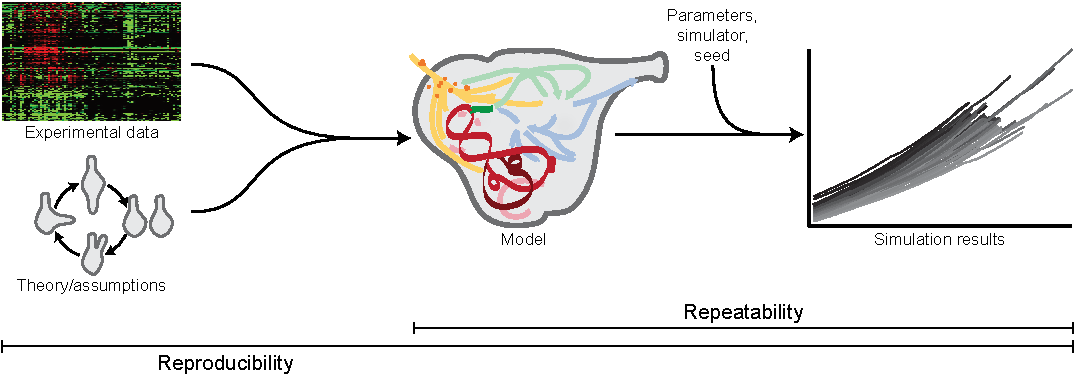
\includegraphics[width=\textwidth]{figure1/figure1}
% where an .eps filename suffix will be assumed under latex,
% and a .pdf suffix will be assumed for pdflatex; or what has been declared
% via \DeclareGraphicsExtensions.
\caption{Model reproducibility refers to derivation from scientific knowledge and the
ability to generate results in a reliable, repeatable manner; Replicability encompasses only the latter concept.}
\label{fig_repro_diagram}
\end{figure*}

\section{Replicability and Reproducibility}

Replicability of a computational model refers to the ability to
re-run a simulation to obtain identical results \cite{easterbrook2014open}.
Reproducibility is a stronger requirement and requires a replicable result as a basis for comparison.

In order for a model to meet our definition of replicability,
it must be capable of regenerating any previous result (such as a published simulation outcome),
even if the simulation is run on a different machine.
As a necessity, this implies that the model make use of purely deterministic numerical solvers
and any pseudorandom processes are driven in a way independent of the host machine or execution context.
We discuss later how this can be achieved.

As shown in Fig. \ref{fig_repro_diagram}, the requirements for replicability are
included in our definition of reproducibility.
This superset structure is largely motivated by validation considerations.
In a typical construction of a model, there will be a series of tests
that cover reduced parts of the model, and provide a means to verify
that the model reproduces the known functions of a system, according to experiment.
These tests also serve as the foundation for independently reconstructing the model.
If the test results cannot be replicated from run to run, the difficulty of reconstruction
increases dramatically, as results can no longer be directly compared but must instead
be compared to some third standard. %on the basis of recapitulating a behavioral metric.
Any behavioral discrepancy between the original model and its reconstruction
then has two possible causes: Algorithmic non-determinism or a deviation in dynamical
behavior, and further investigation is required to rule out one or the other.
This research imposes a burden on model reproduction, and can forestall or even prevent
model reconstruction efforts.

% which are summarized in Fig. \ref{fig_repro_diagram}.
% The theoretical formulation of the model must be well-understood.
% Many mathematical modeling techniques have been applied to biology \cite{gombert2000mathematical}.
% These techniques have been studied extensively and any new techniques will need to be subjected to
% the same degree of scrutiny in order to form a viable foundation for reproducible models.
% For example, the \textit{M. genitalium} model makes use of a Markov chain process in
% transcriptional elongation. The Markov chain represents states of an RNA polymerase:
% free, non-specifically bound to the chromosome, specifically bound to
% the chromosome (i.e. bound at a locus such as a promoter), and actively transcribing.
% The transition matrix for these states is a necessary detail for reproducibility.

Transparency is essential to achieving reproducibility for complex models.
Making source code publicly available is an important step in this direction \cite{easterbrook2014open}.
However, a systematic framework for transparency is necessary to the continued success of whole-cell modeling.
The ideal goal should be to create a machine-readable database containing information describing the experimental source for all data used in a model.
The \textit{M. genitalium} model has an associated database, WholeCellKB-MG \cite{karr2013wholecellkb},
and we discuss later how to improve the link between data and the processes which consume it in complex models.
%Semantic web technologies such as Resource Description Framework (RDF) can be useful in this capacity, and have been used to successfully express genetic components \cite{galdzicki2014synthetic} using linked data.

% The numerical algorithms used by the simulator must converge on a solution.
% For example, kinetic models define a set of differential equations.
% Assuming boundary conditions are imposed to select a unique solution,
% the numerical result converges to an exact solution which can be reproduced across different simulators.
% % This is possible because the numerical solution of a differential equation
% % converges on the true solution.
% % The convergence of numerical methods has been well-studied for ordinary differential
% % equations \cite{brenan1996numerical}, but convergence of hybrid methods is less well understood.

Experimentally measured single-cell parameters are highly important for whole-cell models.
In the \textit{M. genitalium} model, much of this data comes from the literature.
Over 900 papers and 1,900 experimentally observed parameters were used to construct the model \cite{Karr2012}.
Many of the parameters of the model were based on measurements made in other species \cite{macklin2014future}.
As new measurements are made, more accurate models can be built.
However, this relies on continual improvement in experimental reliability.
One way to achieve this is to deposit experimental results into repositories
containing redundant single-cell data and associated meta-information including
a detailed record of experimental conditions and procedures.
In the model, the sources for various types of experimental data must be preserved,
as well as the rationale behind using them in a particular setting
(e.g. the choice of parameter values).
Future advances may help to automate this process, thus accelerating model development.

\subsection{Current Approaches}

There has been a large effort to address reproducibility and replicability in computational biology.
The state of replicability has improved considerably due to the SED-ML standard \cite{sedml2011}.
However, despite these advances, reproducibility in computational biology remains a challenge \cite{garijo2013quantifying}.

Part of this difficulty can be attributed to gaps in standards.
SED-ML, for example, has good coverage of simulation parameters, but
does not address the determinism or lack thereof in the underlying simulator.
Other concerns, such as data transparency, play an important role that is becoming more apparent.
With the emergence of complex hybrid models, more researchers have noted the increased demand for curated, high quality single-cell measurements in order to improve the current state-of-the-art pathway and genome databases.

Another barrier to reproducibility concerns limited support for standards.
One advantage of representing a model in a standard format such as SBML is the ability
to utilize different simulators.
SBML Level 3 consists of extensions which enable additional
functionality, such as
hierarchical model composition \footnote{http://co.mbine.org/standards/sbml/level-3/version-1/comp/version-1/release-2},
flux balance constraints \footnote{ http://sbml.org/Documents/Specifications/SBML\_Level\_3/Packages/fbc}, and
arrays \footnote{http://sbml.org/Documents/Specifications/SBML\_Level\_3/Packages/arrays}.
While the features offered by these packages are critically important for certain
types of models, not all simulators support them.
As SBML gains highly specialized capabilities, it also becomes fractionated, as
not all researchers have a need for such special-purpose features.
If a model makes use of features outside the SBML Level 3 core specification,
there is a risk of being confined to a niche of the dynamical modeling community.
In this case, the advantage of utilizing SBML, as opposed to an \textit{ad hoc} representation
of the model, is diminished.

One aspect of replicability and reproducibility that is often overlooked is the
behavior of the underlying numeric algorithm.
The timestep of the \textit{M. genitalium} model bears a relation to the timestep
of classical solvers such as Runge-Kutta, but the convergence properties of the hybrid model
are much more complex.
% Given the novelty of whole-cell modeling it is not unexpected that such numerical
% questions have been heretofore unanswered
Whereas no detailed study has currently been performed on how the timestep affects
the whole-cell model's long-term dynamical behavior, for reproducibility purposes it is
an important factor. If a small perturbation has the ability to drastically
affect the simulation results, it is more difficult to reproduce the model.
If, however, the model exhibits robust convergence behavior, then it is
possible for multiple reproductions of the model to arrive at the same results.
Indeed, this is an important property of standards development, as exploited by
the SBML test suite \footnote{http://sbml.org/Software/SBML\_Test\_Suite}.

% \subsection{Replicability Requirements}
%
% % A computer program is a predefined sequence of instructions.
% % In simple applications, provided that a program starts in the same state and reads the same
% % data each time it is run, the output should be constant.
% % In practice, software may fail to meet this expectation.
% % This behavior can be caused by algorithmic design.
%
% % Strictly speaking, most modern computers are designed to be deterministic
% % when viewed from a holistic perspective.
% % % Even software such as the SPIN model checker \cite{holzmann2004spin}, which is designed to
% % % simulate non-determinism, runs on a deterministic host.
% % However, an individual program itself represents a subset of the computer,
% % and when viewed in isolation it may appear to exhibit non-deterministic behavior.
%
% Whether or not such apparent non-determinism (hereafter, simply non-determinism)
% is problematic depends on the application.
% For example, exhaustive methods (such as database queries) do not rely on the order
% in which elements are enumerated.
% However, in greedy methods non-determinism can lead to different output, even
% when the input is the same.
% % Nevertheless, there has been an increasing tendency to deviate from determinism
% % in modern software.
%
% Therefore, in order to achieve replicability, it is necessary to ensure
% algorithmic determinism given the initial state (seed values) for the random number generators used.

\subsection{Determinism and Replicability}

Replicability is a useful tool in studying reproducibility.
If the output of a simulator cannot be replicated, it becomes
difficult to make any objective statement about the accuracy of the
underlying model.

Many modern programming practices make use of non-determinism, with
multithreading and memory layout being two major culprits.
This inherent non-determinism in the software makes replicability
impossible.
Systems biologists need to be aware of these issues insofar as they
can lead to non-replicability of a model.
Therefore, we discuss approaches from computer science which
have been used to successfully eliminate non-determinism
in software.

Non-determinism in most software comes from two sources:

\begin{itemize}
\item Concurrency and synchronization
\item Memory layout
\end{itemize}

Concurrency can be a result of threading, or it can arise from
asynchronous input/output callbacks. In both cases, as well as with memory layout,
the non-determinism
can be seen as the result
of program interaction with the operating system.
The essential motif in this case is an interaction of a subsystem
with a larger system in which it is embedded.
When the subsystem is studied in isolation, the influence of the larger
system becomes a perturbation which cannot be accounted for or controlled by
the subsystem. The apparent ``non-determinism'' in these cases
is due to failing to account for all state information.
This is an important theme (and challenge) in the context of whole-cell modeling,
as we will discuss later. % quantum density matrix analogy

While threading, asynchronous operations, and memory layout all contribute
to non-determinism of software,
concurrency due to threading has received considerable attention in the literature.
This is perhaps due to an increasing push to exploit multi-core CPUs,
and the fact that concurrency is seen as the culprit of ``Heisenbugs,''
(errors which manifest themselves non-deterministically)
although memory layout and asynchronicity also exhibit such problems.

Two systems that have been proposed to eliminate non-determinism in threading
are C{\small ORE}D{\small ET} \cite{bergan2010coredet} and D{\small THREADS} \cite{liu2011dthreads}.
C{\small ORE}D{\small ET} is a framework and library for compiling C/C++ programs
using the LLVM compiler framework such that the generated machine code operates deterministically.
D{\small THREADS} is a replacement for the standard UNIX Pthreads library.
Both of these systems operate by preventing the sharing of information between
threads during a parallel phase, and allowing sharing and synchronization
in a deterministic way in a serial phase.
This biphasic structure imposes an overhead on the operation of the threading
system, but these approaches nevertheless show performance comparable to native
threading in many benchmarked cases \cite{liu2011dthreads}, indicating that they show
practical promise.

Both C{\small ORE}D{\small ET} and D{\small THREADS} also
feature deterministic memory allocation. In the case of D{\small THREADS},
this is achieved through a specially implemented memory allocator,
whereas in C{\small ORE}D{\small ET} it is achieved through compiling the
memory allocator itself with the C{\small ORE}D{\small ET} framework.

\subsection{Replicability and Reproducibility of the Whole-Cell Model}

The \textit{M. genitalium} whole-cell model \cite{Karr2012} consists of
28 submodels.
Each submodel represents a physiological process of the cell
and each is based on a mathematical biological modeling technique
(e.g. ODEs, Boolean networks, and flux balance analysis).

The model cannot be encoded in current standards.
One reason for this is that no standards for hybrid modeling currently exist.
While the hierarchical model composition package in SBML Level 3 does allow
for the encoding of multiple submodels, the extension relies on the ability
to flatten the resulting composite model to a single larger model.
Thus, it is not possible to represent modules which run independently
and synchronize at regular timesteps, as is the case in the \textit{M. genitalium} whole-cell model.

The \textit{M. genitalium} model makes use of features outside of SBML Level 3 core,
such as rule-based and stoichiometric methods.
While this is not a barrier to encoding the model in SBML \textit{per se}, the lack
of a single simulator which supports all of the necessary extensions
prevents such a model from being simulated.

The WholeCellKB-MG database \cite{karr2013wholecellkb} contains manually curated data upon which the
\textit{M. genitalium} model is built. The database includes detailed
information on genes, proteins, and reaction pathways identified in the literature.
This is important for reproducibility purposes, as WholeCellKB-MG presents
data in an easily accessible format and helps to document the assumptions
inherent in the \textit{M. genitalium} model.
However, details regarding the dynamical models used to simulate cellular
processes are not included in the database, and in such cases recourse to
source code-level documentation is necessary.
The scope of the \textit{M. genitalium} whole-cell model places it in an
unusual category, where not all mechanistic details of the model are explained in primary
publications. Hence, it highlights the need for summarizing the
dynamical processes in a model without requiring the user to be an expert on the model's
source code.

SBML was developed in part to address these concerns. As a declarative language
for modeling, SBML distills out the processes of a model from the implementation.
The complexity of simulation is then shifted to separate software.
SBML itself has become highly complex, and includes many packages which
have sparse or no support from simulators.
In this sense, it ceases to be a universal language for model exchange.

SBGN also aims to provide a summary of a model, though it is centered
around human readability as opposed to software.
SBGN is useful in the sense that it provides a standard visual representation
of a process, but this representation is produced and used exclusively by humans,
and human error plays a role just as with documentation embedded in source code comments.

\subsection{Standardization Efforts}

% Standardization of the \textit{M. genitalium} whole-cell model \cite{Karr2012}
% was the topic of a workshop in Rostock, Germany from March 9-13, 2015.
% The workshop was organized by subdividing the participants into teams,
% each of which focused on one of the 28 submodels of the whole-cell model
% \hl{[Waltemath(same issue)?]}.
%
% Recalling that (in this paper) reproducibility refers to the ability to
% reimplement a model and still recover the same predictions.
% Recreating exact numerical replicas is not a requirement for this definition
% of reproducibility.
%
% An additional goal of the workshop was to assess and improve the current
% condition of standards within the biological modeling community.
% This in fact became the dominant consideration in many of the teams,
% including the transcription team, which one of us (J.K. Medley)
% was a member of.

% SBML is the de facto standard for encoding biological models \cite{hucka2003systems},
% and encoding the processes represented in the \textit{M. genitalium}
% submodels represented a major area of focus.
% The main difficulty in arriving at a satisfactory SBML representation
% of the transcription submodel is due to the use of a Markov chain
% process for modeling transcriptional elongation.
% In the whole-cell model, an RNA polymerase may be in one of four states:
% free, non-specifically bound to the chromosome, specifically bound to
% the chromosome (i.e. bound at a locus such as a promoter), and actively transcribing.
% Transitions between these states are governed by various factors
% (transitioning from bound to active, for example, requires a sigma factor).

The \textit{M. genitalium} whole-cell model poses several novel challenges for standards.
The most significant is supporting a hybrid modeling approach.
The integration of the submodels (as in \textit{M. genitalium}) is not currently
addressed by standards. In order to be replicable, it must be done deterministically.
A simulation involves running each submodel independently. At each time step,
the submodels are synchronized and the shared variables are updated.
The whole-cell model coordinates this synchronization and partitions resources such as ATP
among the submodels.
This process is not unlike a multithreaded software system where each thread performs
a specific task. The serial execution of a program can be designed to be deterministic.
Likewise, the submodels of the whole-cell model are designed in such a way that
they are individually replicable. The seed for the pseudorandom number generator
used in the whole-cell model was recorded in order to allow replication of simulation results.

The integration of these disparate modeling techniques poses distinct challenges.
Much in the same way that multithreaded programming greatly complicates
determinism in software, integration of submodels complicates the behavior
of the whole-cell model.
Using systems like C{\small ORE}D{\small ET} and D{\small THREADS}, it is possible
to achieve deterministic behavior of a computer program which uses threads.
It is instructive to consider whether the same approach can be applied to whole-cell
modeling, and indeed the \textit{M. genitalium} whole-cell model already displays
some hallmarks of deterministic frameworks, such as the biphasic structure if its timestep.
This suggests that technologies such as C{\small ORE}D{\small ET} and D{\small THREADS}
can offer insights into how to integrate a hybrid model in a replicable way.

Besides hybrid modeling, the \textit{M. genitalium} model highlights the use of
standards as self-documenting. In a system composed purely of reactions,
SBML specifies the minimum amount of information required for reproduction - the rate laws and
boundary conditions. The complexities of numerical integration are not handled by the SBML encoding.
However, many recent SBML Level 3 packages have tended to focus on
structural features of the model which organize elements or
improve simulator performance.
This represents a shift away from the element description of the bare mathematical
entities of the model. This shift may be necessary in some cases to enable
simulation of certain types of models, but it detracts from the ability
of standards to be self-documenting, and detract from reproducibility.

% SBML models the occupancy of discrete states, and while the RNA polymerase states
% are discrete and enumerable, the various states of transcript elongation
% represent an explosion of states. Each gene of length $n$ admits $n$ states
% at different stages of elongation.
% This sheer number of states, one for each \textit{M. genitalium's}
% 580,076 base pairs, overwhelms most SBML
% simulators.
% Furthermore, an even greater number of states would be required to model additional physiological processes during transcription,
% such as the early binding of ribosomes before the transcript is released
% by the polymerase (a detail which is not currently incorporated into the
% \textit{M. genitalium} model).
% For this reason, discrete elongation states are not a scalable solution.
% There may be hope for rule-based modeling of such systems using the SBML
% multi package \footnote{http://sbml.org/Documents/Specifications/SBML\_Level\_3/Packages/multi}, but the essential focus here is not the current limitations
% of standards, but rather on methods enabling robust reproduction of results,
% with the view that standards will follow practice.

% The Markov chain describing the transcription process can, for example,
% be readily simulated using Gillespie's algorithm \cite{gillespie1977exact}
% with rate laws representing relative state transition probabilities.
% The limitations of state space size notwithstanding, this approach renders
% the transcriptional process amenable to reproduction within SBML.

% needed in second column of first page if using \IEEEpubid
%\IEEEpubidadjcol

% \subsubsection{Subsubsection Heading Here}
% Subsubsection text here.


% An example of a floating figure using the graphicx package.
% Note that \label must occur AFTER (or within) \caption.
% For figures, \caption should occur after the \includegraphics.
% Note that IEEEtran v1.7 and later has special internal code that
% is designed to preserve the operation of \label within \caption
% even when the captionsoff option is in effect. However, because
% of issues like this, it may be the safest practice to put all your
% \label just after \caption rather than within \caption{}.
%
% Reminder: the "draftcls" or "draftclsnofoot", not "draft", class
% option should be used if it is desired that the figures are to be
% displayed while in draft mode.
%

% Note that IEEE typically puts floats only at the top, even when this
% results in a large percentage of a column being occupied by floats.


% An example of a double column floating figure using two subfigures.
% (The subfig.sty package must be loaded for this to work.)
% The subfigure \label commands are set within each subfloat command,
% and the \label for the overall figure must come after \caption.
% \hfil is used as a separator to get equal spacing.
% Watch out that the combined width of all the subfigures on a 
% line do not exceed the text width or a line break will occur.
%
%\begin{figure*}[!t]
%\centering
%\subfloat[Case I]{\includegraphics[width=2.5in]{box}%
%\label{fig_first_case}}
%\hfil
%\subfloat[Case II]{\includegraphics[width=2.5in]{box}%
%\label{fig_second_case}}
%\caption{Simulation results for the network.}
%\label{fig_sim}
%\end{figure*}
%
% Note that often IEEE papers with subfigures do not employ subfigure
% captions (using the optional argument to \subfloat[]), but instead will
% reference/describe all of them (a), (b), etc., within the main caption.
% Be aware that for subfig.sty to generate the (a), (b), etc., subfigure
% labels, the optional argument to \subfloat must be present. If a
% subcaption is not desired, just leave its contents blank,
% e.g., \subfloat[].


% An example of a floating table. Note that, for IEEE style tables, the
% \caption command should come BEFORE the table and, given that table
% captions serve much like titles, are usually capitalized except for words
% such as a, an, and, as, at, but, by, for, in, nor, of, on, or, the, to
% and up, which are usually not capitalized unless they are the first or
% last word of the caption. Table text will default to \footnotesize as
% IEEE normally uses this smaller font for tables.
% The \label must come after \caption as always.
%
%\begin{table}[!t]
%% increase table row spacing, adjust to taste
%\renewcommand{\arraystretch}{1.3}
% if using array.sty, it might be a good idea to tweak the value of
% \extrarowheight as needed to properly center the text within the cells
%\caption{An Example of a Table}
%\label{table_example}
%\centering
%% Some packages, such as MDW tools, offer better commands for making tables
%% than the plain LaTeX2e tabular which is used here.
%\begin{tabular}{|c||c|}
%\hline
%One & Two\\
%\hline
%Three & Four\\
%\hline
%\end{tabular}
%\end{table}


% Note that the IEEE does not put floats in the very first column
% - or typically anywhere on the first page for that matter. Also,
% in-text middle ("here") positioning is typically not used, but it
% is allowed and encouraged for Computer Society conferences (but
% not Computer Society journals). Most IEEE journals/conferences use
% top floats exclusively. 
% Note that, LaTeX2e, unlike IEEE journals/conferences, places
% footnotes above bottom floats. This can be corrected via the
% \fnbelowfloat command of the stfloats package.




\section{Conclusion}
% Biology involves the study of complex systems.
% In order to c useful models, it is necessary to use approximations.
% These approximations are representative of the underlying physical
% system at various degrees of granularity in terms of time and space.
% The accuracy of models derived from such approximations may be influenced
% by lack of pertinent data, computational limitations, or lack of
% understanding of the modeled system.
%
% In the modeling community, we must recognize that the assumptions which
% are used in a complex model (such as the \textit{M. genitalium} whole-cell model)
% form a scientific inquiry: The assumptions used in the model are
% essentially a hypothesis, and the test of this hypothesis is whether
% these assumptions capture all relevant dynamical information
% at the time and space scale of the simulation.
% This can be answered by testing the model's predictions against other
% models and also against non-training data.
%
% Ultimately, transparency, numerical robustness, and documentation all influence the reproducibility
% of a model. Large, complex models such as the \textit{M. genitalium} whole-cell model
% help emphasize these needs.
% Other fields have also encountered these issues in different context and have
% responded by building standards and tools to satisfy these needs.
% Due to the complexity of biological systems, the field of computational biology
% may well need to push beyond the solutions devised in the past.
% In this report, we have highlighted several areas where reproducibility may be improved.
% Technological breakthroughs in these areas will enable more rapid progress in whole-cell modeling.
%
% Sharing of data and source code is important for ensuring model reproducibility.
% However, the ability of these resources to be self-documenting varies inversely
% with complexity.
% Having a special purpose standard is a key factor in building reproducible models.
% Special purpose standards can encapsulate the mathematical behavior of a model
% with a minimum of extraneous information, thereby allowing others to
% quickly and independently understand, use, validate, and refine a model.

The \textit{M. genitalium} whole-cell model has pushed the frontier of hybrid modeling
and revealed new challenges for reproducibility.
These challenges include curating and maintaining repositories of single-cell data,
documenting model assumptions explicitly, and running simulations in a replicable way.
The sheer complexity of the \textit{M. genitalium} model necessitates the
automation of tasks which are commonly done manually.
Continued development of whole-cell models will require software which is capable
of linking data to model parameter values.

% \appendices
% \section{Proof of the First Zonklar Equation}
% Appendix one text goes here.

% Can use something like this to put references on a page
% by themselves when using endfloat and the captionsoff option.
\ifCLASSOPTIONcaptionsoff
  \newpage
\fi

\bibliographystyle{IEEEtran}
\bibliography{IEEEabrv,model_reproducibility}

%%%%%%%%%%%%%%%%%%%%%
%% biography section
%%%%%%%%%%%%%%%%%%%%%
\begin{IEEEbiography}[{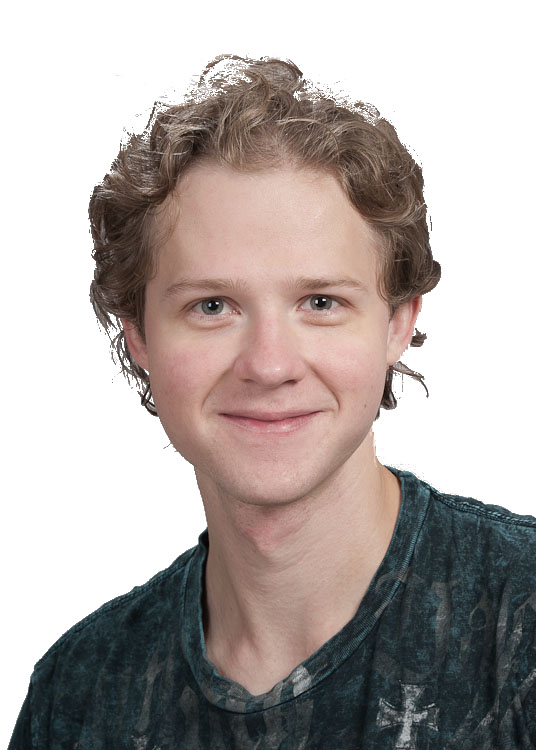
\includegraphics[width=1in,height=1.25in,clip,keepaspectratio]{photos/medley.jpg}}]{J. Kyle Medley}
is currently pursuing a Ph.D. in Bioengineering from the University of Washington, USA.
His research interests include modeling dynamical biophysical processes such as
metabolism and gene expression regulation.
He currently develops libRoadRunner, a software package used to simulate dynamical models encoded in SBML.
\end{IEEEbiography}

\begin{IEEEbiography}[{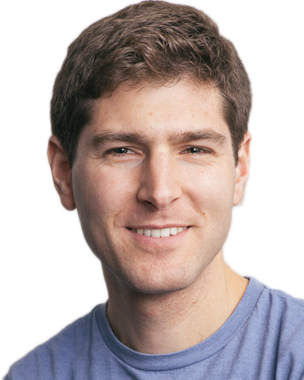
\includegraphics[width=1in,height=1.25in,clip,keepaspectratio]{photos/karr.jpg}}]{Jonathan R. Karr}
received his Ph.D. in Biophysics and M.S. in Medicine from Stanford University, USA in 2014 and his B.S.s in Physics and Brain \& Cognitive Sciences from the Massachusetts Institute of Technology, USA in 2006. Currently, Dr. Karr is a Fellow at the Icahn School of Medicine at Mount Sinai, USA. His research focuses on the development of comprehensive whole-cell computational models and their applications to bioengineering and medicine.
\end{IEEEbiography}

\begin{IEEEbiography}[{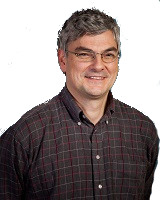
\includegraphics[width=1in,height=1.25in,clip,keepaspectratio]{photos/sauro.jpg}}]{Herbert M. Sauro}
received his Ph.D. in Computational Biochemistry from Oxford Brooks University, UK in 1985, his M.S. in Biological Computation from the University of York, UK, in 1982, and his B.S. in Biochemistry/Microbiology from the University of Canterbury, UK in 1981. He is currently an Associate Professor in the Department of Bioengineering at the University of Washington, USA. His lab develops the next generation of biological modeling and simulation software to help meet the needs of \textit{in silico} studies of biological systems.
\end{IEEEbiography}

\vfill

\end{document}